\documentclass[]{article}
\usepackage{lmodern}
\usepackage{amssymb,amsmath}
\usepackage{ifxetex,ifluatex}
\usepackage{fixltx2e} % provides \textsubscript
\ifnum 0\ifxetex 1\fi\ifluatex 1\fi=0 % if pdftex
  \usepackage[T1]{fontenc}
  \usepackage[utf8]{inputenc}
\else % if luatex or xelatex
  \ifxetex
    \usepackage{mathspec}
  \else
    \usepackage{fontspec}
  \fi
  \defaultfontfeatures{Ligatures=TeX,Scale=MatchLowercase}
\fi
% use upquote if available, for straight quotes in verbatim environments
\IfFileExists{upquote.sty}{\usepackage{upquote}}{}
% use microtype if available
\IfFileExists{microtype.sty}{%
\usepackage{microtype}
\UseMicrotypeSet[protrusion]{basicmath} % disable protrusion for tt fonts
}{}
\usepackage[margin=1in]{geometry}
\usepackage{hyperref}
\hypersetup{unicode=true,
            pdftitle={treelength\_share.R},
            pdfauthor={Amy},
            pdfborder={0 0 0},
            breaklinks=true}
\urlstyle{same}  % don't use monospace font for urls
\usepackage{color}
\usepackage{fancyvrb}
\newcommand{\VerbBar}{|}
\newcommand{\VERB}{\Verb[commandchars=\\\{\}]}
\DefineVerbatimEnvironment{Highlighting}{Verbatim}{commandchars=\\\{\}}
% Add ',fontsize=\small' for more characters per line
\usepackage{framed}
\definecolor{shadecolor}{RGB}{248,248,248}
\newenvironment{Shaded}{\begin{snugshade}}{\end{snugshade}}
\newcommand{\AlertTok}[1]{\textcolor[rgb]{0.94,0.16,0.16}{#1}}
\newcommand{\AnnotationTok}[1]{\textcolor[rgb]{0.56,0.35,0.01}{\textbf{\textit{#1}}}}
\newcommand{\AttributeTok}[1]{\textcolor[rgb]{0.77,0.63,0.00}{#1}}
\newcommand{\BaseNTok}[1]{\textcolor[rgb]{0.00,0.00,0.81}{#1}}
\newcommand{\BuiltInTok}[1]{#1}
\newcommand{\CharTok}[1]{\textcolor[rgb]{0.31,0.60,0.02}{#1}}
\newcommand{\CommentTok}[1]{\textcolor[rgb]{0.56,0.35,0.01}{\textit{#1}}}
\newcommand{\CommentVarTok}[1]{\textcolor[rgb]{0.56,0.35,0.01}{\textbf{\textit{#1}}}}
\newcommand{\ConstantTok}[1]{\textcolor[rgb]{0.00,0.00,0.00}{#1}}
\newcommand{\ControlFlowTok}[1]{\textcolor[rgb]{0.13,0.29,0.53}{\textbf{#1}}}
\newcommand{\DataTypeTok}[1]{\textcolor[rgb]{0.13,0.29,0.53}{#1}}
\newcommand{\DecValTok}[1]{\textcolor[rgb]{0.00,0.00,0.81}{#1}}
\newcommand{\DocumentationTok}[1]{\textcolor[rgb]{0.56,0.35,0.01}{\textbf{\textit{#1}}}}
\newcommand{\ErrorTok}[1]{\textcolor[rgb]{0.64,0.00,0.00}{\textbf{#1}}}
\newcommand{\ExtensionTok}[1]{#1}
\newcommand{\FloatTok}[1]{\textcolor[rgb]{0.00,0.00,0.81}{#1}}
\newcommand{\FunctionTok}[1]{\textcolor[rgb]{0.00,0.00,0.00}{#1}}
\newcommand{\ImportTok}[1]{#1}
\newcommand{\InformationTok}[1]{\textcolor[rgb]{0.56,0.35,0.01}{\textbf{\textit{#1}}}}
\newcommand{\KeywordTok}[1]{\textcolor[rgb]{0.13,0.29,0.53}{\textbf{#1}}}
\newcommand{\NormalTok}[1]{#1}
\newcommand{\OperatorTok}[1]{\textcolor[rgb]{0.81,0.36,0.00}{\textbf{#1}}}
\newcommand{\OtherTok}[1]{\textcolor[rgb]{0.56,0.35,0.01}{#1}}
\newcommand{\PreprocessorTok}[1]{\textcolor[rgb]{0.56,0.35,0.01}{\textit{#1}}}
\newcommand{\RegionMarkerTok}[1]{#1}
\newcommand{\SpecialCharTok}[1]{\textcolor[rgb]{0.00,0.00,0.00}{#1}}
\newcommand{\SpecialStringTok}[1]{\textcolor[rgb]{0.31,0.60,0.02}{#1}}
\newcommand{\StringTok}[1]{\textcolor[rgb]{0.31,0.60,0.02}{#1}}
\newcommand{\VariableTok}[1]{\textcolor[rgb]{0.00,0.00,0.00}{#1}}
\newcommand{\VerbatimStringTok}[1]{\textcolor[rgb]{0.31,0.60,0.02}{#1}}
\newcommand{\WarningTok}[1]{\textcolor[rgb]{0.56,0.35,0.01}{\textbf{\textit{#1}}}}
\usepackage{graphicx,grffile}
\makeatletter
\def\maxwidth{\ifdim\Gin@nat@width>\linewidth\linewidth\else\Gin@nat@width\fi}
\def\maxheight{\ifdim\Gin@nat@height>\textheight\textheight\else\Gin@nat@height\fi}
\makeatother
% Scale images if necessary, so that they will not overflow the page
% margins by default, and it is still possible to overwrite the defaults
% using explicit options in \includegraphics[width, height, ...]{}
\setkeys{Gin}{width=\maxwidth,height=\maxheight,keepaspectratio}
\IfFileExists{parskip.sty}{%
\usepackage{parskip}
}{% else
\setlength{\parindent}{0pt}
\setlength{\parskip}{6pt plus 2pt minus 1pt}
}
\setlength{\emergencystretch}{3em}  % prevent overfull lines
\providecommand{\tightlist}{%
  \setlength{\itemsep}{0pt}\setlength{\parskip}{0pt}}
\setcounter{secnumdepth}{0}
% Redefines (sub)paragraphs to behave more like sections
\ifx\paragraph\undefined\else
\let\oldparagraph\paragraph
\renewcommand{\paragraph}[1]{\oldparagraph{#1}\mbox{}}
\fi
\ifx\subparagraph\undefined\else
\let\oldsubparagraph\subparagraph
\renewcommand{\subparagraph}[1]{\oldsubparagraph{#1}\mbox{}}
\fi

%%% Use protect on footnotes to avoid problems with footnotes in titles
\let\rmarkdownfootnote\footnote%
\def\footnote{\protect\rmarkdownfootnote}

%%% Change title format to be more compact
\usepackage{titling}

% Create subtitle command for use in maketitle
\newcommand{\subtitle}[1]{
  \posttitle{
    \begin{center}\large#1\end{center}
    }
}

\setlength{\droptitle}{-2em}

  \title{treelength\_share.R}
    \pretitle{\vspace{\droptitle}\centering\huge}
  \posttitle{\par}
    \author{Amy}
    \preauthor{\centering\large\emph}
  \postauthor{\par}
      \predate{\centering\large\emph}
  \postdate{\par}
    \date{Mon Apr 8 14:06:25 2019}


\begin{document}
\maketitle

\begin{Shaded}
\begin{Highlighting}[]
\KeywordTok{library}\NormalTok{(ape)}
\KeywordTok{library}\NormalTok{(phytools)}
\end{Highlighting}
\end{Shaded}

\begin{verbatim}
## Loading required package: maps
\end{verbatim}

\begin{Shaded}
\begin{Highlighting}[]
\KeywordTok{library}\NormalTok{(ggplot2)}
\KeywordTok{library}\NormalTok{(reshape2)}

\CommentTok{###################################################################}
\CommentTok{#ompA}
\NormalTok{ompA_trees<-}\KeywordTok{read.nexus}\NormalTok{(}\DataTypeTok{file=}\StringTok{"ompA_trees1.nex"}\NormalTok{)}
\NormalTok{ompA_treelength<-}\KeywordTok{numeric}\NormalTok{()}
\ControlFlowTok{for}\NormalTok{ (i }\ControlFlowTok{in} \DecValTok{1}\OperatorTok{:}\KeywordTok{length}\NormalTok{(ompA_trees))\{}
\NormalTok{  ompA_treelength[i]<-}\KeywordTok{sum}\NormalTok{(ompA_trees[[i]]}\OperatorTok{$}\NormalTok{edge.length)}
\NormalTok{\}}

\NormalTok{ompA_trees2<-}\KeywordTok{read.nexus}\NormalTok{(}\DataTypeTok{file=}\StringTok{"ompA_trees2.nex"}\NormalTok{)}
\NormalTok{ompA_treelength2<-}\KeywordTok{numeric}\NormalTok{()}
\ControlFlowTok{for}\NormalTok{ (i }\ControlFlowTok{in} \DecValTok{1}\OperatorTok{:}\KeywordTok{length}\NormalTok{(ompA_trees2))\{}
\NormalTok{  ompA_treelength2[i]<-}\KeywordTok{sum}\NormalTok{(ompA_trees2[[i]]}\OperatorTok{$}\NormalTok{edge.length)}
\NormalTok{\}}
\CommentTok{#sanity check for expected differences}
\KeywordTok{mean}\NormalTok{(ompA_treelength2)}
\end{Highlighting}
\end{Shaded}

\begin{verbatim}
## [1] 1.769525
\end{verbatim}

\begin{Shaded}
\begin{Highlighting}[]
\KeywordTok{mean}\NormalTok{(ompA_treelength)}
\end{Highlighting}
\end{Shaded}

\begin{verbatim}
## [1] 1.774128
\end{verbatim}

\begin{Shaded}
\begin{Highlighting}[]
\CommentTok{#Concatenate lengths from the two runs}
\NormalTok{ompA<-}\KeywordTok{c}\NormalTok{(ompA_treelength,ompA_treelength2)}
\CommentTok{#View(ompA)}

\CommentTok{###################################################################}
\CommentTok{#CP}
\NormalTok{CP_trees<-}\KeywordTok{read.nexus}\NormalTok{(}\DataTypeTok{file=}\StringTok{"CP_trees1.nex"}\NormalTok{)}
\NormalTok{CP_treelength<-}\KeywordTok{numeric}\NormalTok{()}
\ControlFlowTok{for}\NormalTok{ (i }\ControlFlowTok{in} \DecValTok{1}\OperatorTok{:}\KeywordTok{length}\NormalTok{(CP_trees))\{}
\NormalTok{  CP_treelength[i]<-}\KeywordTok{sum}\NormalTok{(CP_trees[[i]]}\OperatorTok{$}\NormalTok{edge.length)}
\NormalTok{\}}

\NormalTok{CP_trees2<-}\KeywordTok{read.nexus}\NormalTok{(}\DataTypeTok{file=}\StringTok{"CP_trees2.nex"}\NormalTok{)}
\NormalTok{CP_treelength2<-}\KeywordTok{numeric}\NormalTok{()}
\ControlFlowTok{for}\NormalTok{ (i }\ControlFlowTok{in} \DecValTok{1}\OperatorTok{:}\KeywordTok{length}\NormalTok{(CP_trees2))\{}
\NormalTok{  CP_treelength2[i]<-}\KeywordTok{sum}\NormalTok{(CP_trees2[[i]]}\OperatorTok{$}\NormalTok{edge.length)}
\NormalTok{\}}
\CommentTok{#sanity check for expected differences}
\KeywordTok{mean}\NormalTok{(CP_treelength2)}
\end{Highlighting}
\end{Shaded}

\begin{verbatim}
## [1] 1.695029
\end{verbatim}

\begin{Shaded}
\begin{Highlighting}[]
\KeywordTok{mean}\NormalTok{(CP_treelength)}
\end{Highlighting}
\end{Shaded}

\begin{verbatim}
## [1] 1.687781
\end{verbatim}

\begin{Shaded}
\begin{Highlighting}[]
\CommentTok{# Concatenate lengths from the two runs}
\NormalTok{CP<-}\KeywordTok{c}\NormalTok{(CP_treelength,CP_treelength2,}\OtherTok{NA}\NormalTok{,}\OtherTok{NA}\NormalTok{)}
\CommentTok{#View(CP)}


\CommentTok{######################################################################}
\CommentTok{#Analysis:}
\NormalTok{Rates<-}\KeywordTok{data.frame}\NormalTok{(ompA, CP)}
\KeywordTok{head}\NormalTok{(Rates)}
\end{Highlighting}
\end{Shaded}

\begin{verbatim}
##       ompA       CP
## 1 1.740000 1.656377
## 2 4.494645 1.655845
## 3 2.955226 1.557088
## 4 2.870168 1.625642
## 5 2.443038 1.600637
## 6 1.942515 1.639293
\end{verbatim}

\begin{Shaded}
\begin{Highlighting}[]
\NormalTok{data<-}\KeywordTok{melt}\NormalTok{(Rates)}
\end{Highlighting}
\end{Shaded}

\begin{verbatim}
## No id variables; using all as measure variables
\end{verbatim}

\begin{Shaded}
\begin{Highlighting}[]
\KeywordTok{head}\NormalTok{(data)}
\end{Highlighting}
\end{Shaded}

\begin{verbatim}
##   variable    value
## 1     ompA 1.740000
## 2     ompA 4.494645
## 3     ompA 2.955226
## 4     ompA 2.870168
## 5     ompA 2.443038
## 6     ompA 1.942515
\end{verbatim}

\begin{Shaded}
\begin{Highlighting}[]
\KeywordTok{ggplot}\NormalTok{(data,}\KeywordTok{aes}\NormalTok{(}\DataTypeTok{x=}\NormalTok{value, }\DataTypeTok{fill=}\NormalTok{variable)) }\OperatorTok{+}\StringTok{ }
\StringTok{  }\KeywordTok{geom_density}\NormalTok{(}\DataTypeTok{alpha=}\FloatTok{0.25}\NormalTok{) }\OperatorTok{+}
\StringTok{  }\KeywordTok{xlim}\NormalTok{(}\DecValTok{1}\NormalTok{,}\FloatTok{2.5}\NormalTok{)}
\end{Highlighting}
\end{Shaded}

\begin{verbatim}
## Warning: Removed 6 rows containing non-finite values (stat_density).
\end{verbatim}

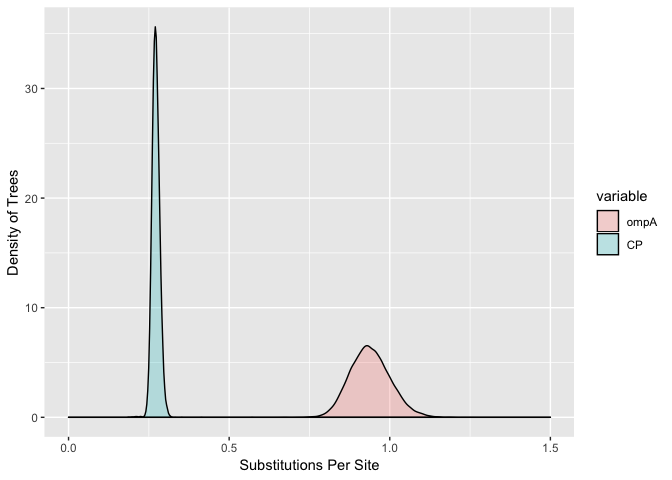
\includegraphics{treelength_share_files/figure-latex/unnamed-chunk-1-1.pdf}

\begin{Shaded}
\begin{Highlighting}[]
\KeywordTok{hist}\NormalTok{(CP)}
\end{Highlighting}
\end{Shaded}

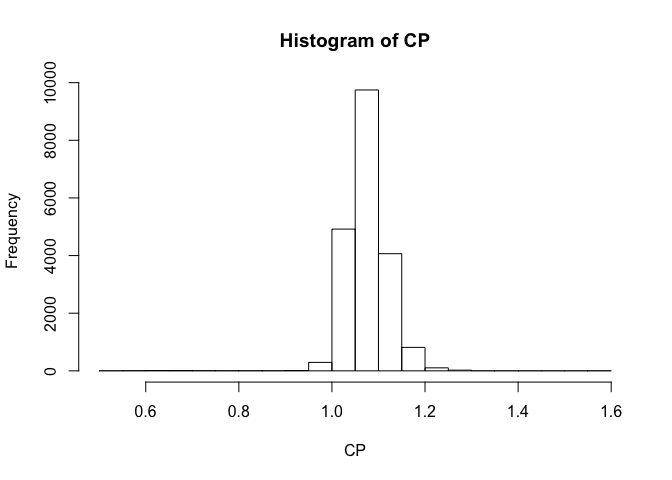
\includegraphics{treelength_share_files/figure-latex/unnamed-chunk-1-2.pdf}

\begin{Shaded}
\begin{Highlighting}[]
\KeywordTok{mean}\NormalTok{(CP,}\DataTypeTok{na.rm=}\OtherTok{TRUE}\NormalTok{)}
\end{Highlighting}
\end{Shaded}

\begin{verbatim}
## [1] 1.691405
\end{verbatim}

\begin{Shaded}
\begin{Highlighting}[]
\KeywordTok{mean}\NormalTok{(ompA)}
\end{Highlighting}
\end{Shaded}

\begin{verbatim}
## [1] 1.771827
\end{verbatim}

\begin{Shaded}
\begin{Highlighting}[]
\KeywordTok{hist}\NormalTok{(ompA)}
\end{Highlighting}
\end{Shaded}

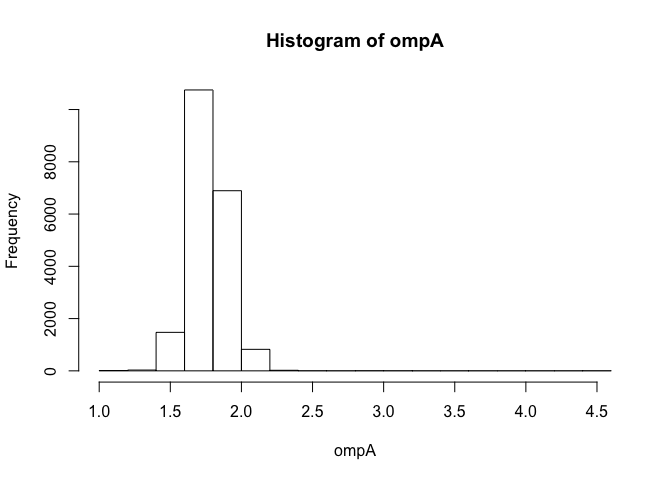
\includegraphics{treelength_share_files/figure-latex/unnamed-chunk-1-3.pdf}


\end{document}
